% !TEX program = xelatex
% 공통수학2 · Ⅲ. 함수와 그래프 · 1. 함수 · 03 역함수 · 2/2차시
% 학생용 활동지 (답안 없음)
\documentclass[11pt,a4paper]{article}
\usepackage{kotex}
\usepackage{iftex}
\ifPDFTeX\else
  \setmainhangulfont{Noto Serif CJK KR}
  \setsanshangulfont{Noto Sans CJK KR}
\fi
\usepackage[margin=2.1cm]{geometry}
\usepackage{parskip}
\usepackage{enumitem}
\usepackage{array}
\usepackage{tabularx}
\usepackage{xcolor}
\usepackage{amssymb}
\usepackage{tikz}
\usepackage[most]{tcolorbox}
\usepackage{fancyhdr}
\usepackage{titlesec}

\definecolor{goldc}{HTML}{B07C22}
\definecolor{goldstrong}{HTML}{8A5F16}
\definecolor{indigoc}{HTML}{2B3B57}
\definecolor{indigosoft}{HTML}{6E82A6}
\definecolor{linec}{HTML}{D6DACB}
\definecolor{surface2}{HTML}{E4E8DC}
\definecolor{writeline}{HTML}{C7CCBA}
\definecolor{inksoft}{HTML}{52604F}

\titleformat{\section}{\normalfont\sffamily\bfseries\large\color{indigoc}}{\thesection}{0.6em}{}
\titlespacing{\section}{0pt}{14pt}{6pt}
\newtcolorbox{goalbox}{enhanced, breakable, colback=white, colframe=goldc, boxrule=0.5pt, leftrule=3pt, arc=2pt, left=10pt, right=10pt, top=8pt, bottom=8pt}
\newtcolorbox{sheetbox}{enhanced, breakable, colback=white, colframe=linec, boxrule=0.6pt, arc=3pt, left=11pt, right=11pt, top=9pt, bottom=9pt}
\newcommand{\writespace}[1]{%
  \par\nobreak\vspace{3pt}
  \foreach \n in {1,...,#1} {%
    \noindent\textcolor{writeline}{\rule{\linewidth}{0.4pt}}\par\vspace{0.62cm}%
  }
}
\newcommand{\fillblank}[1]{\makebox[#1]{\hrulefill}}
\pagestyle{fancy}\fancyhf{}\renewcommand{\headrulewidth}{0pt}
\fancyfoot[L]{\footnotesize\color{inksoft} 공통수학2 · 2026학년도 2학기 · 지평선고등학교}
\fancyfoot[R]{\footnotesize\color{inksoft} 다음 시간 --- 중단원 마무리(함수)}

\newcommand{\blankgraph}{%
  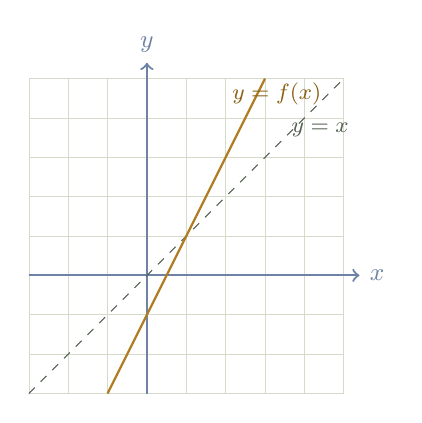
\begin{tikzpicture}[scale=0.5]
    \draw[step=1cm, linec, very thin] (-3,-3) grid (5,5);
    \draw[->, thick, indigosoft] (-3,0) -- (5.4,0) node[right, font=\small]{$x$};
    \draw[->, thick, indigosoft] (0,-3) -- (0,5.4) node[above, font=\small]{$y$};
    \draw[dashed, inksoft] (-3,-3) -- (5,5);
    \node[font=\footnotesize, inksoft] at (4.4,3.7) {$y=x$};
    \draw[thick, goldc, domain=-1:3] plot(\x,{2*\x-1});
    \node[font=\footnotesize, goldstrong] at (3.3,4.6) {$y=f(x)$};
  \end{tikzpicture}}

\begin{document}

\noindent
\begin{minipage}[b]{0.62\linewidth}
  {\sffamily\footnotesize\color{indigosoft} 공통수학2 · Ⅲ. 함수와 그래프 · 1. 함수}\\[2pt]
  {\sffamily\bfseries\Large 03 역함수 \textperiodcentered\ 37차시}
\end{minipage}\hfill
\begin{minipage}[b]{0.36\linewidth}
  \raggedleft\small\color{inksoft}
  반\ \fillblank{1.6cm} \quad 번호\ \fillblank{1.6cm}\\[4pt]
  이름\ \fillblank{3.6cm}
\end{minipage}

\vspace{4pt}
\noindent{\color{goldc}\rule{\linewidth}{2.2pt}}
\vspace{10pt}

\begin{goalbox}
\textbf{오늘의 목표}\\
함수와 역함수의 그래프가 직선 $y=x$에 대하여 대칭임을 이해하고, 역함수의 그래프를 그리며 교점을 구할 수 있다.
\vspace{4pt}
\small\color{inksoft}
$\square$ 자신 있음 \quad $\square$ 조금 헷갈림 \quad $\square$ 처음 봄 \hfill (수업 전 나의 상태에 표시)
\end{goalbox}

\section{생각 열기 --- 대칭이동 다시 보기}

\begin{sheetbox}
15차시에서 배운 것을 떠올려 보자. 점 $(a,b)$를 직선 $y=x$에 대하여 대칭이동하면 그 점의 좌표는 \fillblank{2cm}가 된다.

\vspace{6pt}
만약 점 $(3,7)$이 함수 $y=f(x)$의 그래프 위에 있다면, 즉 $f(3)=7$이라면, 역함수의 정의에 따라 $f^{-1}(7)=\fillblank{1.4cm}$이다. 그렇다면 점 $(7,3)$은 어떤 함수의 그래프 위에 있다고 할 수 있을지 써 보자.
\writespace{2}
\end{sheetbox}

\section{개념 정리 --- 역함수의 그래프}

\begin{sheetbox}
함수 $y=f(x)$의 그래프 위의 점 $(a,b)$는 역함수 $y=f^{-1}(x)$의 그래프 위의 점 $(\ \fillblank{1cm}\ ,\ \fillblank{1cm}\ )$에 대응한다. 따라서 두 그래프는 직선 \fillblank{1.6cm}에 대하여 서로 \fillblank{1.6cm}이다.

\vspace{8pt}
\textbf{예제} --- $f(x)=2x-1$의 그래프를 이용해 역함수 $f^{-1}(x)=\dfrac{x+1}{2}$의 그래프를 그려 보자. (직선 $y=x$에 대하여 대칭이동)

\vspace{4pt}
\centering \blankgraph
\end{sheetbox}

\section{연습 문제}

\begin{sheetbox}
\raggedright
\textbf{1.} 위 예제의 그래프에 $f^{-1}(x)$의 그래프를 이어서 그리고, 두 그래프의 교점의 좌표를 구하시오.
\writespace{2}

\vspace{4pt}
\textbf{2.} 증가함수 $f(x)=x^3$의 그래프와 그 역함수의 그래프의 교점을 모두 구하시오. (힌트: 증가함수이므로 $f(x)=x$를 풀면 된다.)
\writespace{4}

\vspace{4pt}
\textbf{3.} $f(x)=\dfrac12x+2$의 그래프와 역함수의 그래프가 만나는 점을 구하시오.
\writespace{3}

\vspace{4pt}
\textbf{4. (개념 서술형)} ``함수와 그 역함수의 그래프의 교점은 항상 직선 $y=x$ 위에 있다.''는 문장이 참인지 거짓인지 판단하고, 그 이유(어떤 조건에서 성립하는지)를 서술하시오.
\writespace{4}
\end{sheetbox}

\section{사고의 가시화 --- Connect · Extend · Challenge}

\noindent{\footnotesize\color{inksoft} 오늘 배운 `역함수의 그래프'를 떠올리며 아래 세 칸을 채워 보자.}\\[6pt]
\begin{tabularx}{\linewidth}{@{}XXX@{}}
\textbf{\footnotesize\color{indigoc} Connect --- 무엇과 연결되나?} &
\textbf{\footnotesize\color{indigoc} Extend --- 어디까지 확장됐나?} &
\textbf{\footnotesize\color{indigoc} Challenge --- 아직 궁금한 것은?} \\[4pt]
\end{tabularx}
\noindent
\begin{minipage}[t]{0.32\linewidth}\writespace{3}\end{minipage}\hfill
\begin{minipage}[t]{0.32\linewidth}\writespace{3}\end{minipage}\hfill
\begin{minipage}[t]{0.32\linewidth}\writespace{3}\end{minipage}

\section{마무리 성찰}

\begin{sheetbox}
\begin{minipage}[t]{0.48\linewidth}
{\footnotesize\color{inksoft} 오늘 배운 `역함수의 그래프'를 한 문장으로}
\writespace{2}
\end{minipage}\hfill
\begin{minipage}[t]{0.48\linewidth}
{\footnotesize\color{inksoft} 감사 일기 / 유념 한 줄}
\writespace{2}
\end{minipage}
\end{sheetbox}

\end{document}
